% {\gls{palabra}}
% % pdflatex tooltipy-jaod.tex
%  pdflatex -shell-escape rprtmnsl.tex

\documentclass[12pt]{report}
\usepackage{graphicx}
\usepackage{minted}
\usepackage{python}


\begin{document}

\section{Este es un documento ejemplo}

Con el siguiente documento puedes integrar Python y \LaTeX.

\begin{figure}[H]\centering%[22]{r}[0cm]{0.45\linewidth}
\begin{python}
from pylab import *
	
t = arange(0, 1, 0.1)
ll = 102 + t * 20
plot(t, ll, lw=2.5, label =r'${\theta}_{}^{}(t) $')

xlabel('Tiempo [h]',fontsize=18)
ylabel('Distancia [km]',fontsize=18)
legend(loc=4,fontsize=18)
grid(True)
savefig("figs/vcte-mat-intr.pdf")
print r'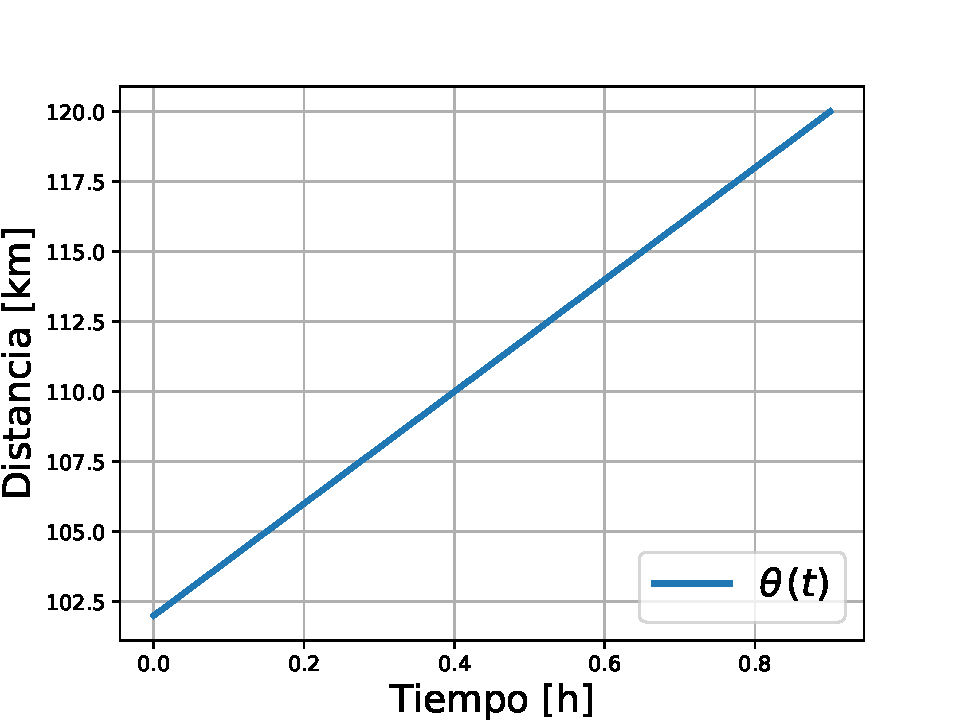
\includegraphics[scale=0.4]{figs/vcte-mat-intr}'

\end{python}
\caption{\label{fig:vcte-mat-intr}
Mostramos la distancia recorrida por un cuerpo en funci\'on del 
tiempo.}
  \end{figure}



\section{Otro ejemplo}


\begin{python}
from pylab import *

text(-.5, 1.1, '$P_i^{}\, (t_{i}^{},v_{i}^{})$',fontsize = 16)
text(0.7, 2.3, '$P_f^{} \,(t_{f}^{},v_{f}^{})$',fontsize = 16)

axis([-0.5, 2., 0.5, 3.])

t = arange(-.2, 1.7, 0.1)
s = (0.7)*t**2 + 1
ll = 0.98 + t*0.95
plot(t, ll, lw=2.5, label ="$a_{4}^{}(t)$", color='green')
plot(t, s, lw=2.5, label ="$a_{4}^{}(t)$", color='blue')

xlabel(r'Tiempo $[T]$', fontsize = 16)
ylabel(r'Velocidad $\frac{[L]}{[T]}$', fontsize = 16)
grid(True)
axis('equal')
savefig("figs/aaver1.pdf")
print r'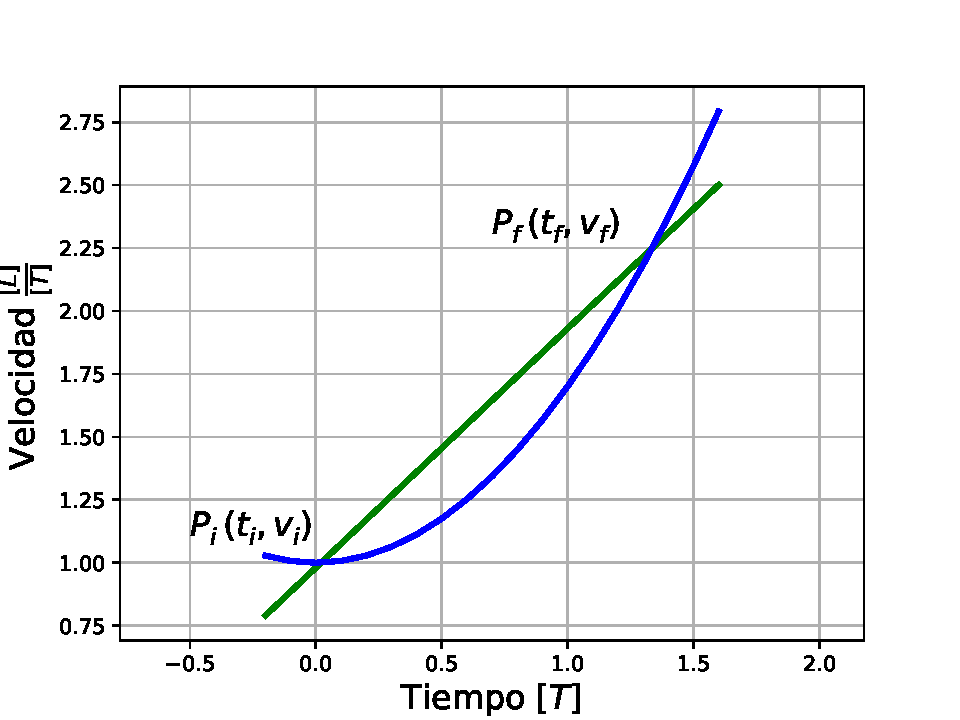
\includegraphics[scale=0.4]{figs/aaver1}'
\end{python}



\section{Una nueva figura}

    \begin{python}
from pyx import *
from pyx.metapost.path import beginknot, endknot, smoothknot, tensioncurve


p1, p2, p3, p4= (0, 0), (2, 0.8), (5, 2.5), (2.5, 2)
p5, p6, p7, p8= (2.6, 0), (5, 0.8), (6, 0.5), (6, 1.5)

closedpath = metapost.path.path([
    smoothknot(*p1),tensioncurve(7.5), 
    smoothknot(*p2), tensioncurve(3.5),
    smoothknot(*p3), tensioncurve(2.5), 
    smoothknot(*p4), tensioncurve(7.5)
])

openpath1 = metapost.path.path([beginknot(*p5), tensioncurve(.5),  endknot(*p8)])

c = canvas.canvas()

l1=path.line(8, 1.5, 6, 1.5)

c.stroke(l1, [style.linewidth.thick,style.linestyle.dashed, color.rgb.blue])

c.stroke(path.line(7, 1, 6, 1),
         [style.linewidth.thick, 
           style.linestyle.dashed, color.rgb.blue,
           deco.earrow([deco.stroked([color.rgb.blue, 
           style.linejoin.round]), deco.filled([color.rgb.blue])], 
           size=0.1)])

c.stroke(closedpath, [trafo.translate(2, 0), style.linewidth.THick, color.rgb.red])

c.stroke(openpath1, [style.linewidth.thick,style.linestyle.dashed, color.rgb.blue])

c.text(6, .45, r"$\vec{v}(t)$")

c.writeEPSfile("figs/imagen")

print r'
\includegraphics[scale=1]{figs/imagen}'
\end{python}

\end{document}

